
%% bare_jrnl_comsoc.tex
%% V1.4b
%% 2015/08/26
%% by Michael Shell
%% see http://www.michaelshell.org/
%% for current contact information.
%%
%% This is a skeleton file demonstrating the use of IEEEtran.cls
%% (requires IEEEtran.cls version 1.8b or later) with an IEEE
%% Communications Society journal paper.
%%
%% Support sites:
%% http://www.michaelshell.org/tex/ieeetran/
%% http://www.ctan.org/pkg/ieeetran
%% and
%% http://www.ieee.org/

%%*************************************************************************
%% Legal Notice:
%% This code is offered as-is without any warranty either expressed or
%% implied; without even the implied warranty of MERCHANTABILITY or
%% FITNESS FOR A PARTICULAR PURPOSE! 
%% User assumes all risk.
%% In no event shall the IEEE or any contributor to this code be liable for
%% any damages or losses, including, but not limited to, incidental,
%% consequential, or any other damages, resulting from the use or misuse
%% of any information contained here.
%%
%% All comments are the opinions of their respective authors and are not
%% necessarily endorsed by the IEEE.
%%
%% This work is distributed under the LaTeX Project Public License (LPPL)
%% ( http://www.latex-project.org/ ) version 1.3, and may be freely used,
%% distributed and modified. A copy of the LPPL, version 1.3, is included
%% in the base LaTeX documentation of all distributions of LaTeX released
%% 2003/12/01 or later.
%% Retain all contribution notices and credits.
%% ** Modified files should be clearly indicated as such, including  **
%% ** renaming them and changing author support contact information. **
%%*************************************************************************


% *** Authors should verify (and, if needed, correct) their LaTeX system  ***
% *** with the testflow diagnostic prior to trusting their LaTeX platform ***
% *** with production work. The IEEE's font choices and paper sizes can   ***
% *** trigger bugs that do not appear when using other class files.       ***                          ***
% The testflow support page is at:
% http://www.michaelshell.org/tex/testflow/



\documentclass[journal,comsoc]{IEEEtran}
%
% If IEEEtran.cls has not been installed into the LaTeX system files,
% manually specify the path to it like:
% \documentclass[journal,comsoc]{../sty/IEEEtran}


\usepackage[T1]{fontenc}% optional T1 font encoding


% Some very useful LaTeX packages include:
% (uncomment the ones you want to load)


% *** MISC UTILITY PACKAGES ***
%
%\usepackage{ifpdf}
% Heiko Oberdiek's ifpdf.sty is very useful if you need conditional
% compilation based on whether the output is pdf or dvi.
% usage:
% \ifpdf
%   % pdf code
% \else
%   % dvi code
% \fi
% The latest version of ifpdf.sty can be obtained from:
% http://www.ctan.org/pkg/ifpdf
% Also, note that IEEEtran.cls V1.7 and later provides a builtin
% \ifCLASSINFOpdf conditional that works the same way.
% When switching from latex to pdflatex and vice-versa, the compiler may
% have to be run twice to clear warning/error messages.






% *** CITATION PACKAGES ***
%
%\usepackage{cite}
% cite.sty was written by Donald Arseneau
% V1.6 and later of IEEEtran pre-defines the format of the cite.sty package
% \cite{} output to follow that of the IEEE. Loading the cite package will
% result in citation numbers being automatically sorted and properly
% "compressed/ranged". e.g., [1], [9], [2], [7], [5], [6] without using
% cite.sty will become [1], [2], [5]--[7], [9] using cite.sty. cite.sty's
% \cite will automatically add leading space, if needed. Use cite.sty's
% noadjust option (cite.sty V3.8 and later) if you want to turn this off
% such as if a citation ever needs to be enclosed in parenthesis.
% cite.sty is already installed on most LaTeX systems. Be sure and use
% version 5.0 (2009-03-20) and later if using hyperref.sty.
% The latest version can be obtained at:
% http://www.ctan.org/pkg/cite
% The documentation is contained in the cite.sty file itself.






% *** GRAPHICS RELATED PACKAGES ***
%
\ifCLASSINFOpdf
  % \usepackage[pdftex]{graphicx}
  % declare the path(s) where your graphic files are
  % \graphicspath{{../pdf/}{../jpeg/}}
  % and their extensions so you won't have to specify these with
  % every instance of \includegraphics
  % \DeclareGraphicsExtensions{.pdf,.jpeg,.png}
\else
  % or other class option (dvipsone, dvipdf, if not using dvips). graphicx
  % will default to the driver specified in the system graphics.cfg if no
  % driver is specified.
  % \usepackage[dvips]{graphicx}
  % declare the path(s) where your graphic files are
  % \graphicspath{{../eps/}}
  % and their extensions so you won't have to specify these with
  % every instance of \includegraphics
  % \DeclareGraphicsExtensions{.eps}
\fi
% graphicx was written by David Carlisle and Sebastian Rahtz. It is
% required if you want graphics, photos, etc. graphicx.sty is already
% installed on most LaTeX systems. The latest version and documentation
% can be obtained at: 
% http://www.ctan.org/pkg/graphicx
% Another good source of documentation is "Using Imported Graphics in
% LaTeX2e" by Keith Reckdahl which can be found at:
% http://www.ctan.org/pkg/epslatex
%
% latex, and pdflatex in dvi mode, support graphics in encapsulated
% postscript (.eps) format. pdflatex in pdf mode supports graphics
% in .pdf, .jpeg, .png and .mps (metapost) formats. Users should ensure
% that all non-photo figures use a vector format (.eps, .pdf, .mps) and
% not a bitmapped formats (.jpeg, .png). The IEEE frowns on bitmapped formats
% which can result in "jaggedy"/blurry rendering of lines and letters as
% well as large increases in file sizes.
%
% You can find documentation about the pdfTeX application at:
% http://www.tug.org/applications/pdftex




% A popular package from the American Mathematical Society that provides
% many useful and powerful commands for dealing with mathematics.
% Do NOT use the amsbsy package under comsoc mode as that feature is
% already built into the Times Math font (newtxmath, mathtime, etc.).
% 
% Also, note that the amsmath package sets \interdisplaylinepenalty to 10000
% thus preventing page breaks from occurring within multiline equations. Use:
\interdisplaylinepenalty=2500
% after loading amsmath to restore such page breaks as IEEEtran.cls normally
% does. amsmath.sty is already installed on most LaTeX systems. The latest
% version and documentation can be obtained at:
% http://www.ctan.org/pkg/amsmath

\usepackage{algorithm}
\usepackage{algpseudocode}
\usepackage{amsmath,amssymb,amsthm,latexsym,paralist, booktabs}
\usepackage{url}
\usepackage[pdftex]{graphicx}
% default pic path
\usepackage{bm}
\usepackage{mathtools}
%\let\oldvec\vec
%\renewcommand{\vec}[1]{\oldvec{\mathit{#1}}}
%\newcommand{\mat}[1]{\mathbf{#1}} % undergraduate algebra version
%\newcommand{\parallelsum}{\mathbin{\!/\mkern-5mu/\!}}
\graphicspath{{pics/}}
\usepackage{upgreek}
% Select a Times math font under comsoc mode or else one will automatically
% be selected for you at the document start. This is required as Communications
% Society journals use a Times, not Computer Modern, math font.
\usepackage[cmintegrals]{newtxmath}
% The freely available newtxmath package was written by Michael Sharpe and
% provides a feature rich Times math font. The cmintegrals option, which is
% the default under IEEEtran, is needed to get the correct style integral
% symbols used in Communications Society journals. Version 1.451, July 28,
% 2015 or later is recommended. Also, do *not* load the newtxtext.sty package
% as doing so would alter the main text font.
% http://www.ctan.org/pkg/newtx
%
% Alternatively, you can use the MathTime commercial fonts if you have them
% installed on your system:
%\usepackage{mtpro2}
%\usepackage{mt11p}
%\usepackage{mathtime}


%\usepackage{bm}
% The bm.sty package was written by David Carlisle and Frank Mittelbach.
% This package provides a \bm{} to produce bold math symbols.
% http://www.ctan.org/pkg/bm





% *** SPECIALIZED LIST PACKAGES ***
%
%\usepackage{algorithmic}
% algorithmic.sty was written by Peter Williams and Rogerio Brito.
% This package provides an algorithmic environment fo describing algorithms.
% You can use the algorithmic environment in-text or within a figure
% environment to provide for a floating algorithm. Do NOT use the algorithm
% floating environment provided by algorithm.sty (by the same authors) or
% algorithm2e.sty (by Christophe Fiorio) as the IEEE does not use dedicated
% algorithm float types and packages that provide these will not provide
% correct IEEE style captions. The latest version and documentation of
% algorithmic.sty can be obtained at:
% http://www.ctan.org/pkg/algorithms
% Also of interest may be the (relatively newer and more customizable)
% algorithmicx.sty package by Szasz Janos:
% http://www.ctan.org/pkg/algorithmicx




% *** ALIGNMENT PACKAGES ***
%
%\usepackage{array}
% Frank Mittelbach's and David Carlisle's array.sty patches and improves
% the standard LaTeX2e array and tabular environments to provide better
% appearance and additional user controls. As the default LaTeX2e table
% generation code is lacking to the point of almost being broken with
% respect to the quality of the end results, all users are strongly
% advised to use an enhanced (at the very least that provided by array.sty)
% set of table tools. array.sty is already installed on most systems. The
% latest version and documentation can be obtained at:
% http://www.ctan.org/pkg/array


% IEEEtran contains the IEEEeqnarray family of commands that can be used to
% generate multiline equations as well as matrices, tables, etc., of high
% quality.




% *** SUBFIGURE PACKAGES ***
%\ifCLASSOPTIONcompsoc
%  \usepackage[caption=false,font=normalsize,labelfont=sf,textfont=sf]{subfig}
%\else
%  \usepackage[caption=false,font=footnotesize]{subfig}
%\fi
% subfig.sty, written by Steven Douglas Cochran, is the modern replacement
% for subfigure.sty, the latter of which is no longer maintained and is
% incompatible with some LaTeX packages including fixltx2e. However,
% subfig.sty requires and automatically loads Axel Sommerfeldt's caption.sty
% which will override IEEEtran.cls' handling of captions and this will result
% in non-IEEE style figure/table captions. To prevent this problem, be sure
% and invoke subfig.sty's "caption=false" package option (available since
% subfig.sty version 1.3, 2005/06/28) as this is will preserve IEEEtran.cls
% handling of captions.
% Note that the Computer Society format requires a larger sans serif font
% than the serif footnote size font used in traditional IEEE formatting
% and thus the need to invoke different subfig.sty package options depending
% on whether compsoc mode has been enabled.
%
% The latest version and documentation of subfig.sty can be obtained at:
% http://www.ctan.org/pkg/subfig




% *** FLOAT PACKAGES ***
%
%\usepackage{fixltx2e}
% fixltx2e, the successor to the earlier fix2col.sty, was written by
% Frank Mittelbach and David Carlisle. This package corrects a few problems
% in the LaTeX2e kernel, the most notable of which is that in current
% LaTeX2e releases, the ordering of single and double column floats is not
% guaranteed to be preserved. Thus, an unpatched LaTeX2e can allow a
% single column figure to be placed prior to an earlier double column
% figure.
% Be aware that LaTeX2e kernels dated 2015 and later have fixltx2e.sty's
% corrections already built into the system in which case a warning will
% be issued if an attempt is made to load fixltx2e.sty as it is no longer
% needed.
% The latest version and documentation can be found at:
% http://www.ctan.org/pkg/fixltx2e


%\usepackage{stfloats}
% stfloats.sty was written by Sigitas Tolusis. This package gives LaTeX2e
% the ability to do double column floats at the bottom of the page as well
% as the top. (e.g., "\begin{figure*}[!b]" is not normally possible in
% LaTeX2e). It also provides a command:
%\fnbelowfloat
% to enable the placement of footnotes below bottom floats (the standard
% LaTeX2e kernel puts them above bottom floats). This is an invasive package
% which rewrites many portions of the LaTeX2e float routines. It may not work
% with other packages that modify the LaTeX2e float routines. The latest
% version and documentation can be obtained at:
% http://www.ctan.org/pkg/stfloats
% Do not use the stfloats baselinefloat ability as the IEEE does not allow
% \baselineskip to stretch. Authors submitting work to the IEEE should note
% that the IEEE rarely uses double column equations and that authors should try
% to avoid such use. Do not be tempted to use the cuted.sty or midfloat.sty
% packages (also by Sigitas Tolusis) as the IEEE does not format its papers in
% such ways.
% Do not attempt to use stfloats with fixltx2e as they are incompatible.
% Instead, use Morten Hogholm'a dblfloatfix which combines the features
% of both fixltx2e and stfloats:
%
% \usepackage{dblfloatfix}
% The latest version can be found at:
% http://www.ctan.org/pkg/dblfloatfix




%\ifCLASSOPTIONcaptionsoff
%  \usepackage[nomarkers]{endfloat}
% \let\MYoriglatexcaption\caption
% \renewcommand{\caption}[2][\relax]{\MYoriglatexcaption[#2]{#2}}
%\fi
% endfloat.sty was written by James Darrell McCauley, Jeff Goldberg and 
% Axel Sommerfeldt. This package may be useful when used in conjunction with 
% IEEEtran.cls'  captionsoff option. Some IEEE journals/societies require that
% submissions have lists of figures/tables at the end of the paper and that
% figures/tables without any captions are placed on a page by themselves at
% the end of the document. If needed, the draftcls IEEEtran class option or
% \CLASSINPUTbaselinestretch interface can be used to increase the line
% spacing as well. Be sure and use the nomarkers option of endfloat to
% prevent endfloat from "marking" where the figures would have been placed
% in the text. The two hack lines of code above are a slight modification of
% that suggested by in the endfloat docs (section 8.4.1) to ensure that
% the full captions always appear in the list of figures/tables - even if
% the user used the short optional argument of \caption[]{}.
% IEEE papers do not typically make use of \caption[]'s optional argument,
% so this should not be an issue. A similar trick can be used to disable
% captions of packages such as subfig.sty that lack options to turn off
% the subcaptions:
% For subfig.sty:
% \let\MYorigsubfloat\subfloat
% \renewcommand{\subfloat}[2][\relax]{\MYorigsubfloat[]{#2}}
% However, the above trick will not work if both optional arguments of
% the \subfloat command are used. Furthermore, there needs to be a
% description of each subfigure *somewhere* and endfloat does not add
% subfigure captions to its list of figures. Thus, the best approach is to
% avoid the use of subfigure captions (many IEEE journals avoid them anyway)
% and instead reference/explain all the subfigures within the main caption.
% The latest version of endfloat.sty and its documentation can obtained at:
% http://www.ctan.org/pkg/endfloat
%
% The IEEEtran \ifCLASSOPTIONcaptionsoff conditional can also be used
% later in the document, say, to conditionally put the References on a 
% page by themselves.




% *** PDF, URL AND HYPERLINK PACKAGES ***
%
%\usepackage{url}
% url.sty was written by Donald Arseneau. It provides better support for
% handling and breaking URLs. url.sty is already installed on most LaTeX
% systems. The latest version and documentation can be obtained at:
% http://www.ctan.org/pkg/url
% Basically, \url{my_url_here}.




% *** Do not adjust lengths that control margins, column widths, etc. ***
% *** Do not use packages that alter fonts (such as pslatex).         ***
% There should be no need to do such things with IEEEtran.cls V1.6 and later.
% (Unless specifically asked to do so by the journal or conference you plan
% to submit to, of course. )


% correct bad hyphenation here
\hyphenation{op-tical net-works semi-conduc-tor}


\begin{document}
%
% paper title
% Titles are generally capitalized except for words such as a, an, and, as,
% at, but, by, for, in, nor, of, on, or, the, to and up, which are usually
% not capitalized unless they are the first or last word of the title.
% Linebreaks \\ can be used within to get better formatting as desired.
% Do not put math or special symbols in the title.

\title{CSCE 664 Wireless and Mobile Systems\\
Project Proposal}
%
%
% author names and IEEE memberships
% note positions of commas and nonbreaking spaces ( ~ ) LaTeX will not break
% a structure at a ~ so this keeps an author's name from being broken across
% two lines.
% use \thanks{} to gain access to the first footnote area
% a separate \thanks must be used for each paragraph as LaTeX2e's \thanks
% was not built to handle multiple paragraphs
%

\author{\IEEEauthorblockN{Yukun Zeng, Bingqian Jiang}\\
\IEEEauthorblockA{Department of Computer Science and Engineering\\
Texas A\&M University\\
College Station, TX 77840\\
Email: \{yzeng, jiangbingqianj\}@tamu.edu}}

% note the % following the last \IEEEmembership and also \thanks - 
% these prevent an unwanted space from occurring between the last author name
% and the end of the author line. i.e., if you had this:
% 
% \author{....lastname \thanks{...} \thanks{...} }
%                     ^------------^------------^----Do not want these spaces!
%
% a space would be appended to the last name and could cause every name on that
% line to be shifted left slightly. This is one of those "LaTeX things". For
% instance, "\textbf{A} \textbf{B}" will typeset as "A B" not "AB". To get
% "AB" then you have to do: "\textbf{A}\textbf{B}"
% \thanks is no different in this regard, so shield the last } of each \thanks
% that ends a line with a % and do not let a space in before the next \thanks.
% Spaces after \IEEEmembership other than the last one are OK (and needed) as
% you are supposed to have spaces between the names. For what it is worth,
% this is a minor point as most people would not even notice if the said evil
% space somehow managed to creep in.



% The paper headers
\markboth{Journal of \LaTeX\ Class Files,~Vol.~14, No.~8, August~2015}%
{Shell \MakeLowercase{\textit{et al.}}: Bare Demo of IEEEtran.cls for IEEE Communications Society Journals}
% The only time the second header will appear is for the odd numbered pages
% after the title page when using the twoside option.
% 
% *** Note that you probably will NOT want to include the author's ***
% *** name in the headers of peer review papers.                   ***
% You can use \ifCLASSOPTIONpeerreview for conditional compilation here if
% you desire.




% If you want to put a publisher's ID mark on the page you can do it like
% this:
%\IEEEpubid{0000--0000/00\$00.00~\copyright~2015 IEEE}
% Remember, if you use this you must call \IEEEpubidadjcol in the second
% column for its text to clear the IEEEpubid mark.



% use for special paper notices
%\IEEEspecialpapernotice{(Invited Paper)}




% make the title area
\maketitle

% As a general rule, do not put math, special symbols or citations
% in the abstract or keywords.
\begin{abstract}
We consider the problem of scaling mobile cloud benchmark on pay-as-you-go cloud computing platforms like AWS and Google Cloud. The intuition behind such an idea is that a large amount of physical mobile devices are hard to manage and impractical in terms of infrastructure cost. In this paper, we propose to virtualize mobile devices directly on top of Xen, a common virtualization system used in typical public cloud like AWS, this would eradicate the overhead of nested virtualization used in other virtualization solutions like Ravello Systems. As we virtualized mobile cloud in this way, the network connection (virtual I/O in this case) between different virtual devices is totally different from real world scenario where mobile devices are connected through wireless networks, typically WLAN. To obtain a more realistic virtualized environment, we further introduce a virtual router that sits on top of the virtual I/O and is responsible for forwarding, dropping, retransmitting data packets so that we can emulate the wireless network behavior on virtual I/O.
\end{abstract}

% Note that keywords are not normally used for peerreview papers.
\begin{IEEEkeywords}
Virtual Router, Wireless Network Emulation, Virtualized Networking, Virtualization, Mobile Cloud 
\end{IEEEkeywords}






% For peer review papers, you can put extra information on the cover
% page as needed:
% \ifCLASSOPTIONpeerreview
% \begin{center} \bfseries EDICS Category: 3-BBND \end{center}
% \fi
%
% For peerreview papers, this IEEEtran command inserts a page break and
% creates the second title. It will be ignored for other modes.
\IEEEpeerreviewmaketitle
\section{Introduction}
\subsection{Mobile Cloud}
With the development of computing capability, we can now achieve performance simular to personal computer on a portable mobile device. This on the one hand eased our life by providing more complex and useful applications on mobile devices while it also created some dilemmas where massive computing resources fitted into phones, smart bands, etc are left idle and wasted most of the time. People have proposed many mobile cloud solutions that leverage the idle computing resource on those devices and use them to fill in high computing resource demand elsewhere. A lot of efforts have been put into mobile cloud and people have developed different platforms to solve different problems by leveraging idle mobile computing resources, we refer readers to \cite{kumar2010cloud} \cite{dinh2013survey} \cite{fernando2013mobile} for more information about the emerging mobile cloud computing trend. In this paper, we will focus on a mobile cloud platform called Mobile Storm \cite{ning2015mobile}, which is a state-of-the-art platform for distributed stream processing and it is a previous work by LENSS lab.
\subsection{Scalibility Benchmark}
Naturally we can think of scalability as a important metric in evaluation of such platforms, however it's unpractical to probe the platform scalability using dedicated mobile device clusters as it's too expensive and even harder to manage than server clusters. To solve such a problem, we proposed to benchmark those platforms by leveraging the on-demand computing resources provided by state-of-the-art cloud computing platforms like AWS and Google Cloud, i.e., we could build mobile cloud by virtualizing any amount of devices based on our demand thereby testing the platform scalability. This approach does not only fit into the benchmarking of mobile cloud platforms but also is suitable for scaling different tests like probing the max load of an application server by adding more and more mobile devices as clients. However, new problems emerge if we are proceeding this way. In most common scenarios of mobile cloud, devices are usually connected through wireless networks, the backend can be either one server or a cluster and those servers are usually connected by wired networks. A typical example of the Mobile Storm cluster can be found in Fig. \ref{mstorm_network} where we have multiple mobile devices connected to each other as well as the master server through wireless router. However, things get totally different if we tries to virtualize the Mobile Storm cluster in public clouds. As shown in Fig. \ref{virtualized_network}, the virtual mobile devices communicates with each other using virtual I/O. Different virtual devices might be running on the same physical machine or different physical machine, thus the virtual I/O can be either I/O of certain machine or wired network between different machines. Anyhow, such connectivity between virtual devices differs a lot from the actual scenario and we have to find a way to emulate wireless network in the virtualized environment so that we can benchmark in a realistic and scalable fashion. 
\begin{figure}[htbp]
\begin{center}
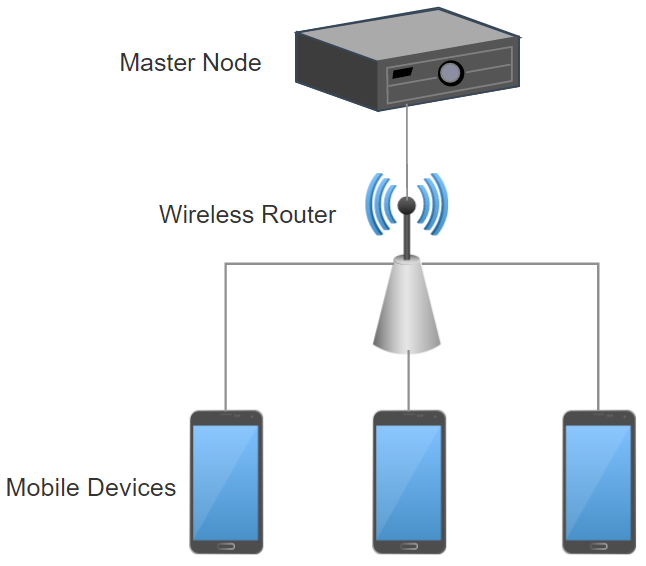
\includegraphics[width=0.8\linewidth]{mstorm_network.png} 
\end{center}	   
\caption{Networking in Actual Mobile Storm Cluster}\label{mstorm_network}
\end{figure}

\begin{figure}[htbp]
\begin{center}
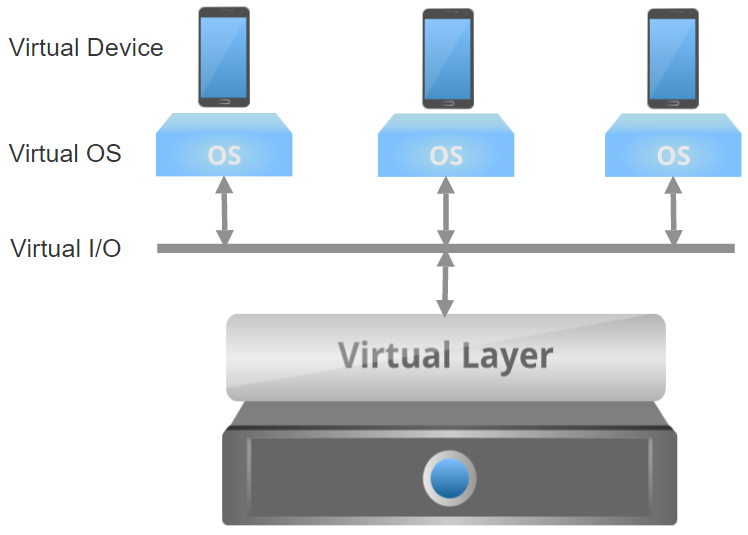
\includegraphics[width=0.8\linewidth]{virtualized_network.png} 
\end{center}	   
\caption{Networking in Virtualized Mobile Storm}\label{virtualized_network}
\end{figure}

\subsection{Existing Solutions}
Though there is a huge trunk of research papers in the field of cloud computing, virtualization as well as mobile clouds, there are few works dedicated to scaling mobile cloud benchmark by virtualizing mobile devices on public clouds, most highly relevant systems are commercialized and available now on market place of AWS. Ravello Systems and Genymotion are two commercial platforms that enable the scalability benchmark for mobile cloud. Ravello Systems enables us to run any virtual machine on any cloud without making any changes through adding a new hypervisor called HVX on top of VMs provided by public cloud platforms. Breaking down the stack of Ravello's solution, as shown in \ref{hvx_diagram}, we can see that we can further run hypervisor on VMs provided by AWS and then run any Virtual Machine on top of the hypervisor. The solutions provided by Genymotion incorporate two aspects, one is to emulate Android x86 OS on top of a host OS in a near-native manner (basically running Android x86 on VirtualBox with all hardware acceleration), the other is to emulate Android OS on demand in public cloud. Genymotion on Demand could similarly provide easy pay-as-you-go Android device virtualization while it's close source and its internal mechanism is rarely discussed. While both solutions can be used for scaling mobile cloud benchmark, none of them can restore the actual wireless network scenario thus cannot guarantee realistic benchmark.
\begin{figure}[htbp]
\begin{center}
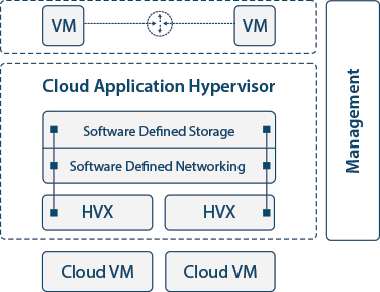
\includegraphics[width=0.8\linewidth]{hvx_diagram.png} 
\end{center}	   
\caption{Destack Ravello System Architecture}\label{hvx_diagram}
\end{figure}

\subsection{Observation and Thoughts}
As shown in Fig. \ref{virtualized_network}, the network of virtual Mobile Storm cluster is based on virtual I/O which is totally different from the wireless network behavior in actual scenario. We assume the virtual I/O is totally reliable. To acquire a wireless-alike environment in the virtualized cluster, our thought is that we might add a router (the router term might not be exactly accurate) on top of virtual I/O to control the traffic. The virtual router is responsible of forwarding data packets to target virtual devices like a wireless link that might generate packet loss, delay, retransmission, basically we wanna incorporate all features of a wireless link as data packets pass through the virtual router.

\subsection{Contribution}
We expect the contributions of this paper as follows:
\begin{itemize}
	\item Propose a new approach of virtualizing mobile cloud directly on top of the Xen virtualization layer, i.e., be able to run android virtual devices cluster on Xen environment, this might also require efforts in virtualized networking as we need to figure out a way for building the interconnectivity between different virtual devices.
	\item Develop a virtual router sitting on top of the virtual I/O to forward data packet and control the transmission between different virtual devices, the final goal of the virtual router is to emulate a wireless network behavior on virtual I/O so that we obtain a realistic environment when virtualizing mobile devices cluster on public clouds.
\end{itemize}

\section{Related Works}
Current solutions for virtualizing mobile devices on cloud mainly include Genymotion  \cite{genymotion} and Ravello Systems. They can both provide pretty good performance for virtualized devices and are highly scalable, but none of them takes common wireless communication paradigms between mobile devices into consideration. This is far from ideal as it is proved in \cite{cen2003end} the wireless network differs a lot from wired network. Both wireless and wired network simulation or emulation have been studied thoroughly in the last decades \cite{zheng2003empower} \cite{judd2005using}. Network virtualization can be realized directly through virtualization systems like VMWare, VirtualBox or Xen, common networking provided by those virtualization systems include NAT, Host-only and bridged. Related works in network virtualization area include \cite{menon2006optimizing} \cite{chowdhury2009network}. However, few researches are dedicated in wireless network emulation in virtualized environment, we need a physical wireless network card on the host machine to acquire wireless behavior for VMs, which is impractical in public cloud. Among all related works, we focus on the following researches as they are the most related ones to our topic:
\subsection{Empower: a network emulator for wireline and wireless networks}
Empower\cite{zheng2003empower} is a distributed network emulation system. It is able to facilitate the emulation of either wireline or wireless networks. In the case when network topology is critical to the underlying network protocol, the emulator could provide specific mechanisms to emulate network topology. Empower can also generate user-defined network conditions and traffic dynamics at packet level.
However,  Empower is specialized in dealing with emulation for wire and wireless networks, which does nothing with cloud service computing. Therefore, we need to move forward for other applications which would fit our concern more.

\subsection{HVX: Virtualizing the Cloud}
HVX \cite{hvx} is a virtualization platform that enables complete abstraction of underlying cloud infrastructure from the application virtual machines. HVX allows deployment of existing VMs into the cloud without any modifications, mobility between the clouds and easy duplication of the entire deployment. HVX can be deployed on almost any existing IaaS cloud. Each instance of the HVX deployment packs in a nested hypervisor, virtual hardware, network and storage configuration. Combined with image store and management APIs, the HVX can be used for the creation of a virtual cloud that utilizes existing cloud provider infrastructure as the hardware rather than using physical servers, switches and storage.However, HVX's virtualization still exhibits the problem that it is unable to simulate the real world wireless communication, which may have higher latency and packets loss rate than wired connection, which HVX adopt at its end.  On the other hand, HVX could be referred as running virtualization on VM, which would significantly slow down the speed. Thus, we may need to propose a better solution to optimize discussed problems. 

\subsection{Genymotion on Demand}
Genymotion \cite{genymotion} is a new cloud-based virtualization platform aimed at Android developers. Running on Amazon Web Services, Genymotion On Demand offers access to the full Android operating environment online. However, Genymotion on Demand is a closed source software whose source code is not published. Therefore, we currently could not be guaranteed whether performance of Genymotion on Demand could satisfy our requirements.

\subsection{Xen}
Xen \cite{barham2003xen} is an x86 virtual machine monitor which allows multiple commodity operating systems to share conventional hardware in a safe and resource managed fashion, but without sacrificing either performance or functionality. This is achieved by providing an idealized virtual machine abstraction to which operating systems such as Linux, BSD and Windows XP, can be ported with minimal effort. The virtualization approach taken by Xen is extremely efficient: it allows operating systems such as Linux and Windows XP to be hosted simultaneously only with a negligible performance overhead --- at most a few percent compared with the unvirtualized case. 

%The advantages of virtualization with Xen comparing to other solutions are as follows:
%\begin{itemize}
%	\item Independence on hardware and the support for different operating systems (both commercial and open source OSs).
%	\item Neither performance nor security and functionalities are sacrificed in Xen to accomodate the requirements of each other.
%	\item Xen offers resource isolation and performance guarantees for VMs running on it without risk of DoS.
%\end{itemize}

Compared with Xen, many other virtualization systems expose a lot of disadvantages. Some require specialized hardware, or cannot support commodity operating systems. Some target $100\%$ binary compatibility at the expense of performance. Others sacrifice security or functionality for speed. Few offer resource isolation or performance guarantees; most provide only best-effort provisioning, risking denial of service. Xen overcomes all above cons, and thus gains popularity with modern public cloud service like AWS. In this paper, we built our virtualized mobile cluster on XenServer, a commercial implementation of Xen. Our research will conducted based on Xen as well. With functions Xen provide, we will further extend and optimize the performance to achieve a faster virtualization environment for real-world wireless cloud service simulation.

\section{Proposed Solution}
\subsection{Virtualizing Mobile Devices in Cloud}
Ravello systems provided solution to run any virtual machine on any cloud without changes to operating systems through nested virtualization, however there will be additional overhead in the 2nd layer of virtualization in terms of processor power, network throughput, etc. Moreover, normal customers of public clouds are serviced directly from the virtualized OS level (i.e., an operating system is immediately installed per request) and they might not have access to nested virtualization as it's a low level setting in Xen which is not commonly exposed by cloud platforms for security considerations. Here in this paper we propose to virtualize Android system directly on top of Xen, which can greatly reduce the overheads. More specifically, we use XenServer as the hypervisor for the physical machine and install Android directly on VMs without any intermediate Linux or Windows system.

\subsection{Wireless Emulator on Virtual I/O}
As we have mentioned before, we can test the scalibility of a mobile cloud platform by leveraging virtualization techniques on public clouds, however, such an approach cannot provide a realistic wireless networking environment as the communication between different virtual devices goes through the virtual I/O, which is either the virtualized system I/O or wired network between different host servers. To better emulate the actual wireless networked mobile cloud platform, we propose a wireless network emulator on top of virtual I/O to virtually control the delivery of data packet between different virtual devices to acquire a network transmission pattern similar to real wireless network system. As shown in Fig. \ref{virtual_router}, the virtual wireless network emulator lies on the virtual I/O layer and is responsible for coordinating the network transmission between different virtual devices. At the current stage, we expect the emulator to be an application on Android, it might exposes some ports to receive or output data packets in the virtualized network, it works by dropping packets and retransmission in a wireless manner. 
\begin{figure}[htbp]
\begin{center}
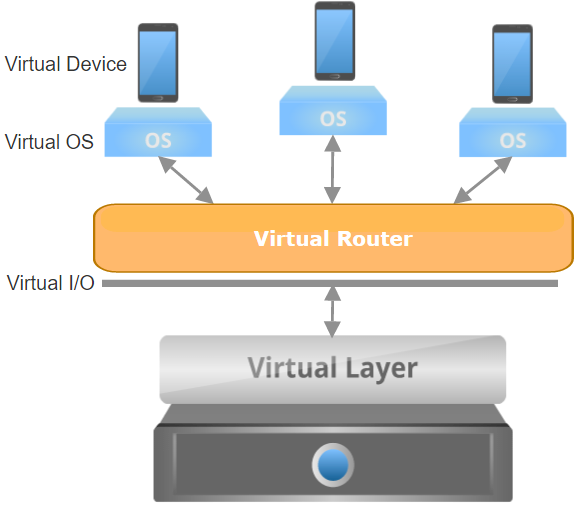
\includegraphics[width=0.8\linewidth]{virtual_router.png} 
\end{center}	   
\caption{Virtual Wireless Network Emulator}\label{virtual_router}
\end{figure}

\subsection{Expected Chanllenges}
Our project is highly challenging in that it incorporates problems in both virtualization and networking, basically we need to find proper approach to achieve the following goals:
\begin{itemize}
	\item Improving virtual device performance: virtual machines are typically much slower than physical machines with the same hardware and software configuration, even with the hardware speedup provided by newly introduced Intel VT-x or AMD-V CPU, which makes the benchmark harder. To reduce the virtualization overhead, we propose to virtualize mobile devices at the lowest level possible and we adopt Android for x86 to acquire better support for desktop CPUs (oppsed to typical Android device CPU like ARM).
	\item Networking in virtualized environment: as we mentioned above, we need to virtualize mobile device cluster using XenServer, however, to the best of our knowledge so far, native network is not provided directly by the virtualized Android system on XenServer, we might have to deal with device driver and figure out a way to network virtual devices in either the same machine or LAN.
	\item Wireless network emulation: though a huge volume of researches have been put into wireless network emulation, here we expect many challenges since we are doing emulation on Android platform and the whole system lies in a virtualized environment, the final implementation of wireless emulation should be a totally different story comparing to previous work.
\end{itemize}
% Can use something like this to put references on a page
% by themselves when using endfloat and the captionsoff option.
\ifCLASSOPTIONcaptionsoff
  \newpage
\fi



% trigger a \newpage just before the given reference
% number - used to balance the columns on the last page
% adjust value as needed - may need to be readjusted if
% the document is modified later
%\IEEEtriggeratref{8}
% The "triggered" command can be changed if desired:
%\IEEEtriggercmd{\enlargethispage{-5in}}

% references section

% can use a bibliography generated by BibTeX as a .bbl file
% BibTeX documentation can be easily obtained at:
% http://mirror.ctan.org/biblio/bibtex/contrib/doc/
% The IEEEtran BibTeX style support page is at:
% http://www.michaelshell.org/tex/ieeetran/bibtex/
%\bibliographystyle{IEEEtran}
% argument is your BibTeX string definitions and bibliography database(s)
%\bibliography{IEEEabrv,../bib/paper}
%
% <OR> manually copy in the resultant .bbl file
% set second argument of \begin to the number of references
% (used to reserve space for the reference number labels box)
\bibliographystyle{IEEEtran}
% argument is your BibTeX string definitions and bibliography database(s)
\bibliography{refs}

% biography section
% 
% If you have an EPS/PDF photo (graphicx package needed) extra braces are
% needed around the contents of the optional argument to biography to prevent
% the LaTeX parser from getting confused when it sees the complicated
% \includegraphics command within an optional argument. (You could create
% your own custom macro containing the \includegraphics command to make things
% simpler here.)
%\begin{IEEEbiography}[{\includegraphics[width=1in,height=1.25in,clip,keepaspectratio]{mshell}}]{Michael Shell}
% or if you just want to reserve a space for a photo:





% that's all folks
\end{document}


